\documentclass[12pt]{article}

\usepackage[utf8]{inputenc}
\usepackage{setspace}
\usepackage{geometry}
\usepackage{graphicx}
\usepackage{caption}
\usepackage{indentfirst}
\usepackage{anyfontsize}
\usepackage{textcomp}
\usepackage{mathtools}
\usepackage{float}
\usepackage{changepage}
\usepackage [english]{babel}
\usepackage [autostyle, english = american]{csquotes}
\usepackage{tabto}
\usepackage{verbatim}
\usepackage{wrapfig}
\usepackage{caption}
\usepackage{subcaption}
\usepackage{stackengine}
\usepackage{scrextend}
\usepackage{xcolor}
\usepackage{booktabs}
\usepackage{bigints}
\usepackage{calc}
\usepackage[nomessages]{fp}


\graphicspath{}
\MakeOuterQuote{"}

\title{Stochastic Modeling}
\author{Geneva Porter \textbf{816408535}}
\date{4 December 2018}

\begin{comment}

\begin{figure}[H]
\centering{\includegraphics[width=10cm]{FILENAME.eps}}
\caption*{\textbf{CAPTION}}
\end{figure}

$\left(\begin{matrix}
11      & 12  \\
21      & 22  \\
\end{matrix}\right)$

\end{comment}

\begin{document}
	
\begin{titlepage}
\maketitle
\thispagestyle{empty}


\begin{center}
	
\large \it San Diego State University 
	
Professor J Mahaffy, Math 636

\end{center}
\end{titlepage}

\section{Invasive Squirrel Species}
The movement of the British red squirrel and the invasive American gray squirrel have been recorded by the British Forestry Commission for the last 45 years. The presence of red squirrels, gray squirrels, both, or neither in a 10$km^2$ region over 2 years was recorded in the following transition matrix:

\begin{center}
	$T=\left(\begin{matrix}
	0.8797 & 0.0382 & 0.0527 & 0.0008 \\
	0.0212 & 0.8002 & 0.0041 & 0.0143 \\
	0.0981 & 0.0273 & 0.8802 & 0.0527 \\
	0.0010 & 0.1343 & 0.0630 & 0.9322 \\
\end{matrix}\right)$, with
$\left(\begin{matrix}
$red squirrels$  \\
$gray squirrels$  \\
$both$ \\
$neither$ \\
\end{matrix}\right)$.
\end{center}

We can find the equilibrium distribution of squirrels by finding the eigenvalues and corresponding eigenvectors of the transition matrix using the MATLAB function $eig()$. Rather than using $T$ to calculate the needed values, $T^5$ was used in order to obtain positive values. While this changes the eigenvalues, it does not change the value or location of the dominant eigenvalue $\lambda_1=1$, nor does it change the value of the normalized eigenvectors. If we know the location of the dominant eigenvalue (in this case, the first column), then we can use the normalized corresponding eigenvector $E$ as our equilibrium distribution:

\vspace{3mm}

\hspace{-9mm}$E=\left(\begin{matrix}
0.2945    &0.5148   &-0.4050   &-0.4360\\
0.0967    &0.0050   & 0.4731   &-0.3857\\
0.5908    &0.2877   & 0.5182   & 0.8131\\
0.7449   &-0.8076   &-0.5862   & 0.0086\\
\end{matrix}\right)\longrightarrow x_e=\left(\begin{matrix}
0.2945\\
0.0967\\
0.5908\\
0.7449\\
\end{matrix}\right)\cdot\dfrac{1}{\sum E_{i,1}}=\left(\begin{matrix}
0.1705\\
0.0560\\
0.3421\\
0.4313\\
\end{matrix}\right)$

\vspace{3mm}

This tells us that 17.05\% of the region is inhabited only by red squirrels, 5.60\% of the region is only inhabited by gray squirrels, 34.21\% of the region is inhabited by both species, and 43.13\% of the region is not inhabited by either species. Over a long period of time, it is not likely that gray squirrels will displace red squirrels, as they dominate only a small percentage of the region.

\section{Frog Habitat Regions}

Suppose an enclosed space is divided into 4 regions of different habitats. The movement of frogs to regions 1 through 4 over the course of a single day is given by the transition matrix:

\begin{center}
	$T = \left(\begin{matrix}
0.42 & 0.16 & 0.19 & 0.16 \\
0.07 & 0.38 & 0.24 & 0.13 \\
0.34 & 0.19 & 0.51 & 0.27 \\
0.17 & 0.27 & 0.06 & 0.44
\\ 
\end{matrix}\right)$
\end{center}

\subsection*{a. Expected Populations}

If we release 100 frogs into region one and observe their movement over 10 days, we can expect the population in each region to change according to the percentage distributions in $T$. We can find these expected changes by multiplying the transition matrix by the initial population for each region, in this case $p_0=(100,0,0,0)^T$, resulting in a population distribution vector. For subsequent days, we can continue to iterate the product of the population vector and the transition matrix. The resulting regional populations might look like this:

\begin{table}[H]
\begin{center}
		\begin{tabular}{|c|c|c|c|c|}
		\hline
		\textbf{}       & \textbf{Region 1} & \textbf{Region 2} & \textbf{Region 3} & \textbf{Region 4} \\ \hline
		\textbf{day 1}  & 42                & 7                 & 34                & 17                \\ \hline
		\textbf{day 2}  & 27.9400           & 15.9700           & 37.5400           & 18.5500           \\ \hline
		\textbf{day 5}  & 23.1737           & 20.6571           & 35.6359           & 20.5333           \\ \hline
		\textbf{day 10} & 23.0600           & 20.6914           & 35.4725           & 20.7762           \\ \hline
	\end{tabular}
\caption*{\textbf{Table 1} Expected Frog Populations}
\end{center}
\end{table}

\subsection*{b. Steady State Distribution}

 We can see that most frogs favor region 3, while regions 2 and 4 are the least favored. The expected population for days 5 and 10 are quite similar as the system moves closer to a steady state. We can verify this by finding the dominant eigenvalue $\lambda_1$ and normalizing its corresponding eigenvector using the same process from problem 1, which gives us:

\begin{center}
	$x_e=\left(\begin{matrix}
0.2306&
0.2069&
0.3547&
0.2078
\end{matrix}\right)^T$
\end{center}

Which is equal to the percent distribution of the frogs on day 10. This vector models the percentage population distribution over long periods of time.

\subsection*{c. Monte Carlo Simulation}

We can obtain similar results by using a Monte Carlo simulation. If we implement this model for 10 days 1,000 times, we can see what the expected population will be at days 1, 2, 5, and 10. The mean population $\bar{x}_{i,j}$ and the standard deviation of the population $\sigma_{i,j}$ in each region for each day are given below:

\begin{table}[H]
\begin{center}
		\begin{tabular}{|l|c|c|c|c|} \hline
$\bar{x}_{i,j}$	&\textbf{ Region 1}	& \textbf{Region 2}	& \textbf{Region 3}	& \textbf{Region 4}	\\ \hline
\textbf{Day 1}&42.038&        6.911 &      34.016  &     17.035\\ \hline
\textbf{Day 2}&28.063  &     15.881   &    37.593  &     18.463\\ \hline
\textbf{Day 3}&22.996 &       20.89  &      35.66   &    20.454\\ \hline
\textbf{Day 4}&23.255  &     20.449   &    35.465  &     20.831\\ \hline
	\end{tabular}
\caption*{\textbf{Table 2} Mean Population over 10 Days}
\end{center}
\end{table}


\begin{table}[H]
\begin{center}
		\begin{tabular}{|l|c|c|c|c|} \hline
		$\sigma_{i,j}$	& \textbf{Region 1}	& \textbf{Region 2}	& \textbf{Region 3}	& \textbf{Region 4}	\\ \hline
		\textbf{Day 1}&        4.943    &   2.5392   &    4.7394    &   3.8492\\  \hline
		\textbf{Day 2}&4.4979  &     3.6205  &     4.7182   &    3.7859\\ \hline
		\textbf{Day 3}&4.3035  &    4.0727   &    4.9304    &  4.0739\\ \hline
		\textbf{Day 4}&4.1648   &    3.8952   &    4.6832   &    4.0965\\ \hline
	\end{tabular}
	\caption*{\textbf{Table 3} Standard Deviation of Population over 10 Days}
\end{center}
\end{table}

The MATLAB code used for these results is found in figure i (Appendix). Notice that $\bar{x}_{4,j}$ is roughly equal to $x_e^T$ (well within one standard deviation), which corresponds to our predictions in parts a and b. This indicates that it is likely that our random distribution simulation will approach the steady-state distribution, given a large enough number of simulations.

\section{Reproduction and Survival}

Here we will examine the population of an animal that lives for four years and reproduces annually.

\subsection*{a. Leslie Matrix Model}

The Leslie matrix model for this species is:

\begin{center}
	$P_{n+1} = \left(\begin{matrix}
	0 & 1.5 & 2.2 & 3.4 \\
	0.4 & 0 & 0 & 0 \\
	0 & 0.7 & 0 & 0 \\
	0 & 0 & .75 & 0
\end{matrix}\right)P_n$
\end{center}

With $P_n$ being a vector representing the populations of each age group (0-1, 1-2, 2-3, and 3-4). This model has a dominant eigenvalue of $\lambda_1=1.2465$, indicating a population growth of 24.65\% each year. If normalize the corresponding eigenvector, we get a steady-state distribution of:

\begin{center}
	$x_e = (0.62129,0.19937,0.11196,0.067368)^T$
\end{center}

With each $x_{e_i}$ corresponding to each age group. To predict population with a constant growth rate, we can assume Malthusian growth behavior to see when this population will double. If we begin with population $p_0$, doubling can be modeled by:

\begin{center}
	$p(t) = p_0\lambda^t=2p_0 \hspace{5mm} \longrightarrow \hspace{5mm} t = \dfrac{ln(2)}{ln\lambda} \approx3.1460$

\end{center}
So the population will double just after 3 years.


\subsection*{b. Harvesting Model}

If the older two age groups are harvested at some rate $\alpha$, the growth rate will decrease and the population distribution will be altered. To find the dominant eigenvalue with this unknown, we can examine the characteristic polynomial of the Leslie Matrix:

\begin{center}
	$\lambda^4-0.6\lambda^2-0.616\alpha\lambda-0.714\alpha^2=0$
\end{center}

Using MATLAB's $root()$ and $solve()$ functions, we can determine that when the principal eigenvalue is equal to 1, $\alpha\approx$0.4325. Therefore, when 43.25\% of the 2-3 and 3-4 age groups are harvested, the growth rate is zero. Our new probability distribution is:

\begin{center}
	$x_e=(0.6409, 0.2563, 0.0776, 0.0252)^T$
\end{center}

Let's say that a typical population with harvesting has 550 individuals in the 3-4 age group. Since these 550 individuals make up 2.52\% of the population, the total population is expected to be 21845.8556. This creates a population distribution of:

\begin{center}
	$p_e=$(14000.2530, 5600.1021, 1695.5005, 550)
\end{center}

With this population, about 2946.1961 individuals age 2-4 are harvested each year.

\section{Bird Reproduction and Survival}

A population of birds were observed over a 4-year period. Researchers categorized the birds into 3 age categories: 0-1 years old, 1-2 years old, and 2+ years old. The Leslie model has the structure:

\begin{center}
	$P_{n+1}=\left(\begin{matrix}
0 & b_2 & b_3\\
s_1 & 0 & 0 \\
0 & s_2 & s_3\\
\end{matrix}\right)P_n$
\end{center}

\subsection*{a. Survival Rates}

We can find the $s$ values by examining the observational data:

\begin{table}[H]
\begin{center}
		\begin{tabular}{|c|c|c|c|c|}
		\hline
		\textbf{Age} & \textbf{Year 1} & \textbf{Year 2} & \textbf{Year 3} & \textbf{Year 4} \\ \hline
		\textbf{0-1} & 175             & 237             & 258             & 311             \\ \hline
		\textbf{1-2} & 42              & 59              & 89              & 92              \\ \hline
		\textbf{2+}  & 97              & 104             & 128             & 145             \\ \hline
	\end{tabular}
\caption*{\textbf{Table 4} Population Over 4 Years}
\end{center}
\end{table}

Birds from the 0-1 age group will be represented by the birds in the 1-2 age group the following year. This results in an average value of $s_1=0.3564$ for the survival rate of the 0-1 aged birds. The 1-2 age group in the first year will be represented by a fraction of the 2+ age group the following year (because of the 2+ age group that survived from the previous year). The researchers observed that the survival rate of the 1-2 age group and the survival rate of the 2+ age group are roughly equal, so $s_2=s_3$. Knowing this, we can calculate the survival rate with the following general equation:

\vspace{3mm}

$(p_{1-2}$ population year$_i)s_3+(p_{2+}$ population year$_i)s_3 = (p_{2+}$ population year$_{i+1})$

\vspace{3mm}

With $p_k$ being the population of a certain age group for year$_i$. Solving this equation for $s_3$ for each year and averaging our results we get $s_2=s_3=0.7339$. We can use the following data to calculate the values for birth rates, $b_2$ and $b_3$:

\begin{table}[H]
	\begin{center}
		\begin{tabular}{|c|c|c|c|c|}
			\hline
			\textbf{Age} & \textbf{Year 1} & \textbf{Year 2} & \textbf{Year 3} & \textbf{Year 4} \\ \hline
			\textbf{1-2} & 38              & 47              & 66              & 74              \\ \hline
			\textbf{2+}  & 199              & 211             & 245             & 293             \\ \hline
		\end{tabular}
		\caption*{\textbf{Table 5} Nesting Over 4 Years}
	\end{center}
\end{table}

We calculate the average birth rates for each age group by taking the number of successful nestings divided by the population for that group for a given year. Taking the average over 4 years, we obtain values of $b_2 = 0.81182$ and $b_3=2.0038$.

\subsection*{b. Leslie Matrix}

We have solved the missing values $b_2, b_3, s_1, and s_2=s_3$. The Leslie matrix for this population is therefore: 

\begin{center}
	$L=\left(\begin{matrix}
0      		&0.81182      & 2.0038 \\
0.35642     &       0     &       0\\
0     		& 0.73389     & 0.73389\\
\end{matrix}\right)$
\end{center}

We can use the Leslie matrix to predict the population change over the course of the next 3 years by multiplying it by the population vector and iterating the results. Table 6 shows the expected populations at years 5, 6, and 7 (given the population observed at year 4):


\begin{table}[H]
	\begin{center}
		\begin{tabular}{|c|c|c|c|}
			\hline
			\textbf{Age} & \textbf{Year 5} & \textbf{Year 6} & \textbf{Year 7} \\ \hline
			\textbf{0-1} & 365.2367       & 438.5118       &524.4678             \\ \hline
			\textbf{1-2} & 110.8465       & 130.1776       &156.2943             \\ \hline
			\textbf{2+}  & 173.9327       &   208.9977       &248.9185             \\ \hline
		\end{tabular}
		\caption*{\textbf{Table 6} Population Over Years 5-7}
	\end{center}
\end{table}

\subsection*{c. Eigenvalues and Eigenvectors}

If we examine the Leslie matrix more closely, we can determine the limiting percent population for each age group. The eigenvalue ($V$) and the eigenvector ($E$) matrices are given by:

\begin{center}
$V = \left(\begin{matrix}
-0.2303            &0          &  0\\
0     &-0.2303           & 0\\
0           & 0       &1.1946\\
\end{matrix}\right)$ and 
	$E = \left(\begin{matrix}
0.7631      &0.7631     & 0.8727\\
-0.2400      & -0.2400      &0.2602\\
0.0095  & 0.0095    &  0.4145\\
\end{matrix}\right)$
\end{center}

We can see that our dominant eigenvalue is 1.1941, so our annual growth rate is 19.41\%. The corresponding eigenvector $E_{i,4}$ gives us a percent population distribution when normalized, resulting in:

\begin{center}
	$x_e=(0.5638, 0.1682, 0.2680)^T$
\end{center}

To find the time when the population will double, we can use the same formula from the previous problem, resulting in a value of $t=3.9071$. The population will double just after 3 years.

\section{E. Coli and Enzyme Reactions}

For this problem, we examine the chemical reactions of enzymatic transformations. Here $S_1$ is a substrate, $S_2$ is an enzyme, $S_3$ is the enzyme-substrate complex, and $S_4$ is the resultant product. The enzymatic transformation of $S_1$ into $S_4$ is given by:

\begin{center}
	$S_1+S_2\hspace{5mm}\underrightarrow{c_1}\hspace{5mm} S_3$
\end{center}

\begin{center}
	$S_3 \hspace{5mm}\underrightarrow{c_2}\hspace{5mm} S_1+S_2$
\end{center}

\begin{center}
	$S_3 \hspace{5mm}\underrightarrow{c_3}\hspace{5mm} S_2+S_4$
\end{center}

\subsection*{a. E. Coli Gillespie Algorithm}

We can model the above enzymatic transformation using a Gillespie algorithm in MATLAB, as shown in the code displayed in figure ii (Appendix). We will examine E. coli and compute its enzymatic transformation using the following values for numbers of molecules ($S_k$) and rate constants ($c_i$):

\begin{center}	
$S_1=500$, $S_2=50$, $S_3=S_4=0$, $c_1=0.002$, $c_2=6\times10^{-5}$, and $c_3=0.08$
\end{center}

Staring with these values, 2 simulations were calculated. Figure 1 below shows the results of these simulations over a time period $t=[0,200]$.

\begin{figure}[H]
	\centering
	\begin{minipage}{.5\textwidth}
		\centering
		\includegraphics[width=8cm]{g1.png}
		\label{fig:test1}
	\end{minipage}%
	\begin{minipage}{.5\textwidth}
		\centering
		\includegraphics[width=8cm]{g2.png}
		\label{fig:test2}
	\end{minipage}
\caption*{\textbf{Figure 1} E. Coli Enzymatic Transformation Model Using Gillespie Algorithm}
\end{figure}

Because the Gillespie Algorithm depends on random number probabilities to determine the likelihood of chemical reactions happening, we see some slight differences in the two graphs above. For simulation no.1, 993 reactions occurred in the given time period, while 1000 reactions occurred when populating simulation no.2. Both see a large initial value of $S_1$ that declines roughly proportionately to the increase of $S_4$. The two values seem to mirror each other along a horizontal line at $\approx230$. Similar behavior is seen in the relationship between $S_2$ and $S_3$. This would indicate that the rate of change of each substance in the pair is opposite in sign, resulting in no net change in the system. There are some temporal differences between the two simulations. Simulation no.1 seems to have overlapping values for each substance (as if some negative time steps occurred) past $t\approx160$. Conversely, simulation no.2 ends just before the $t=200$ mark, indicating that there was a time step that lept forward before landing closer to 200.

\subsection*{b. System of Differential Equations}

The reactions illustrated above can be written as 4 differential equations, one for each substance:

\begin{center}
	$\dfrac{dS_1}{dt}=-S_1S_2c_1+S_3c_2$
\end{center}

\begin{center}
	$\dfrac{dS_2}{dt}=-S_1S_2c_1+S_3c_2+S_3c_3$
\end{center}

\begin{center}
	$\dfrac{dS_3}{dt}=S_1S_2c_1-S_3c_2-S_3c_3$
\end{center}

\begin{center}
	$\dfrac{dS_4}{dt}=S_3c_3$
\end{center}

These equations are an illustration of the Lotka-Volterra model for species competition. We can model these using MATLAB's $ode23()$, as shown in figure 2 below. Simulation no.2 from the previous section is shown as dotted lines for comparison.

We can see that the two models pair up nicely. They both have mirrored pairs $S_1$ with $S_4$ and $S_2$ with $S_3$. Naturally, the Gillespie algorithm model is jagged, as it is has random variance. If we were to run a few thousand simulations and average the results, we would likely see a smoother curve that more closely matches the ODE model.

Previously we discussed how $S_2$ and $S_3$ have equal but opposite rates of change, which is confirmed by examining their derivatives, which add to zero. This indicates that the the value $S_2 + S_3$ is equal to a constant (the antiderivative of zero), in this case 50. Since there must be zero net change in the system by the law of conservation of mass, $S_1$ and $S_4$ must also have equal and opposite rates of change. Therefore, $dS_1/dt+dS_4/dt=0$ and $S_1+S_4$=500.

\begin{figure}[H]
\centering{\includegraphics[width=13cm]{g3.png}}
\caption*{\textbf{Figure 2} E. Coli Enzymatic Transformation Model Using ODEs}
\end{figure}


\subsection*{c. ODE Simplification}

An alternative way to model the above system is given by:

\begin{center}
	$\dfrac{dS_1}{st}=-\dfrac{V_mS_1}{K_m+S_1}$ and $\dfrac{dS_4}{dt}=\dfrac{V_mS_1}{K_m+S_1}$
\end{center}

Here, $V_m$ and $K_m$ are kinetic constants. If we simulate the ODE using these equations, we can compare it with the solutions from our 4-function system. If we minimize the error using MATLAB's $fminsearch()$ function, we get $V_m=4.8247$ and $K_m=89.0255$, with a sum of squared errors of 12588.1459. However, we can significantly reduce that error by slightly altering our initial values. If we begin with $S_1=472.7621$ and $S_4=0.0011$, then we obtain values of $V_m=4.0815$ and $K_m=43.4690$, with  sum of squared errors of 3679.8409. This is much more reasonable, and fairly close to our original initial conditions. 

With the altered initial values, the simplified version of our system is a good fit (figure 3, below). Despite having a smaller amount of substrate to begin with, the curves fit well through most of the plot. Of course, the initial value of $S_1$ and the final value of $S_4$ are the greatest difference between the plots. Also, the simplified version has values that are slightly higher than the full version, due to an equal distribution of weighting for each value. If the values between $t=[20,140]$ were weighted more heavily, then the simplified system would be a better fit.

\begin{figure}[H]
	\centering{\includegraphics[width=13cm]{g4b.png}}
	\caption*{\textbf{Figure 3} Simplified Version of Michaelis-Menten Reactions}
\end{figure}

\subsection*{d. Dimensional Stuff}

So far we have been using the unit of "molecules" to describe the initial conditions of our systems. If we were to provide standard international units to these values, then we would want to describe our initial substrate and enzyme amounts in terms of $mole/liters$. This would be a simple unit conversion:

\begin{center}
	$S_k\cdot\dfrac{1mole}{6.0221\times10^{23}}\cdot\dfrac{1}{7\times10^{-19}liters}=1.1624\times10^{-4}S_km/l$
\end{center}

This would give us $S_1=5.8119\times10^{-2}m/l$ and $S_2=5.8119\times10^{-3}m/l$. These values do not depend on time. If we are to consider the kinetic constant $K_m$, we would see that it must also be in units of $m/l$ (and thus must be multiplied by our conversion factor as well). This gives us $K_m=5.0527\times10^{-3}m/l$. Our units for $V_m$, however, must be dependent on time. Logic tells us that the derivative of a non-autonomous function will be expressed as some rate with respect to time. We can assume that $V_m$ is in units of $msec^{-1}$, so conversion to seconds can be accomplished by multiplying by $10^{-3}$. Therefore, $V_m=4.0815\times10^{-3}s^{-1}$.

So, that's it I guess.






\pagebreak

\section*{Appendix}

\subsection*{MATLAB code for frog populations}

\begin{figure}[H]
	\centering{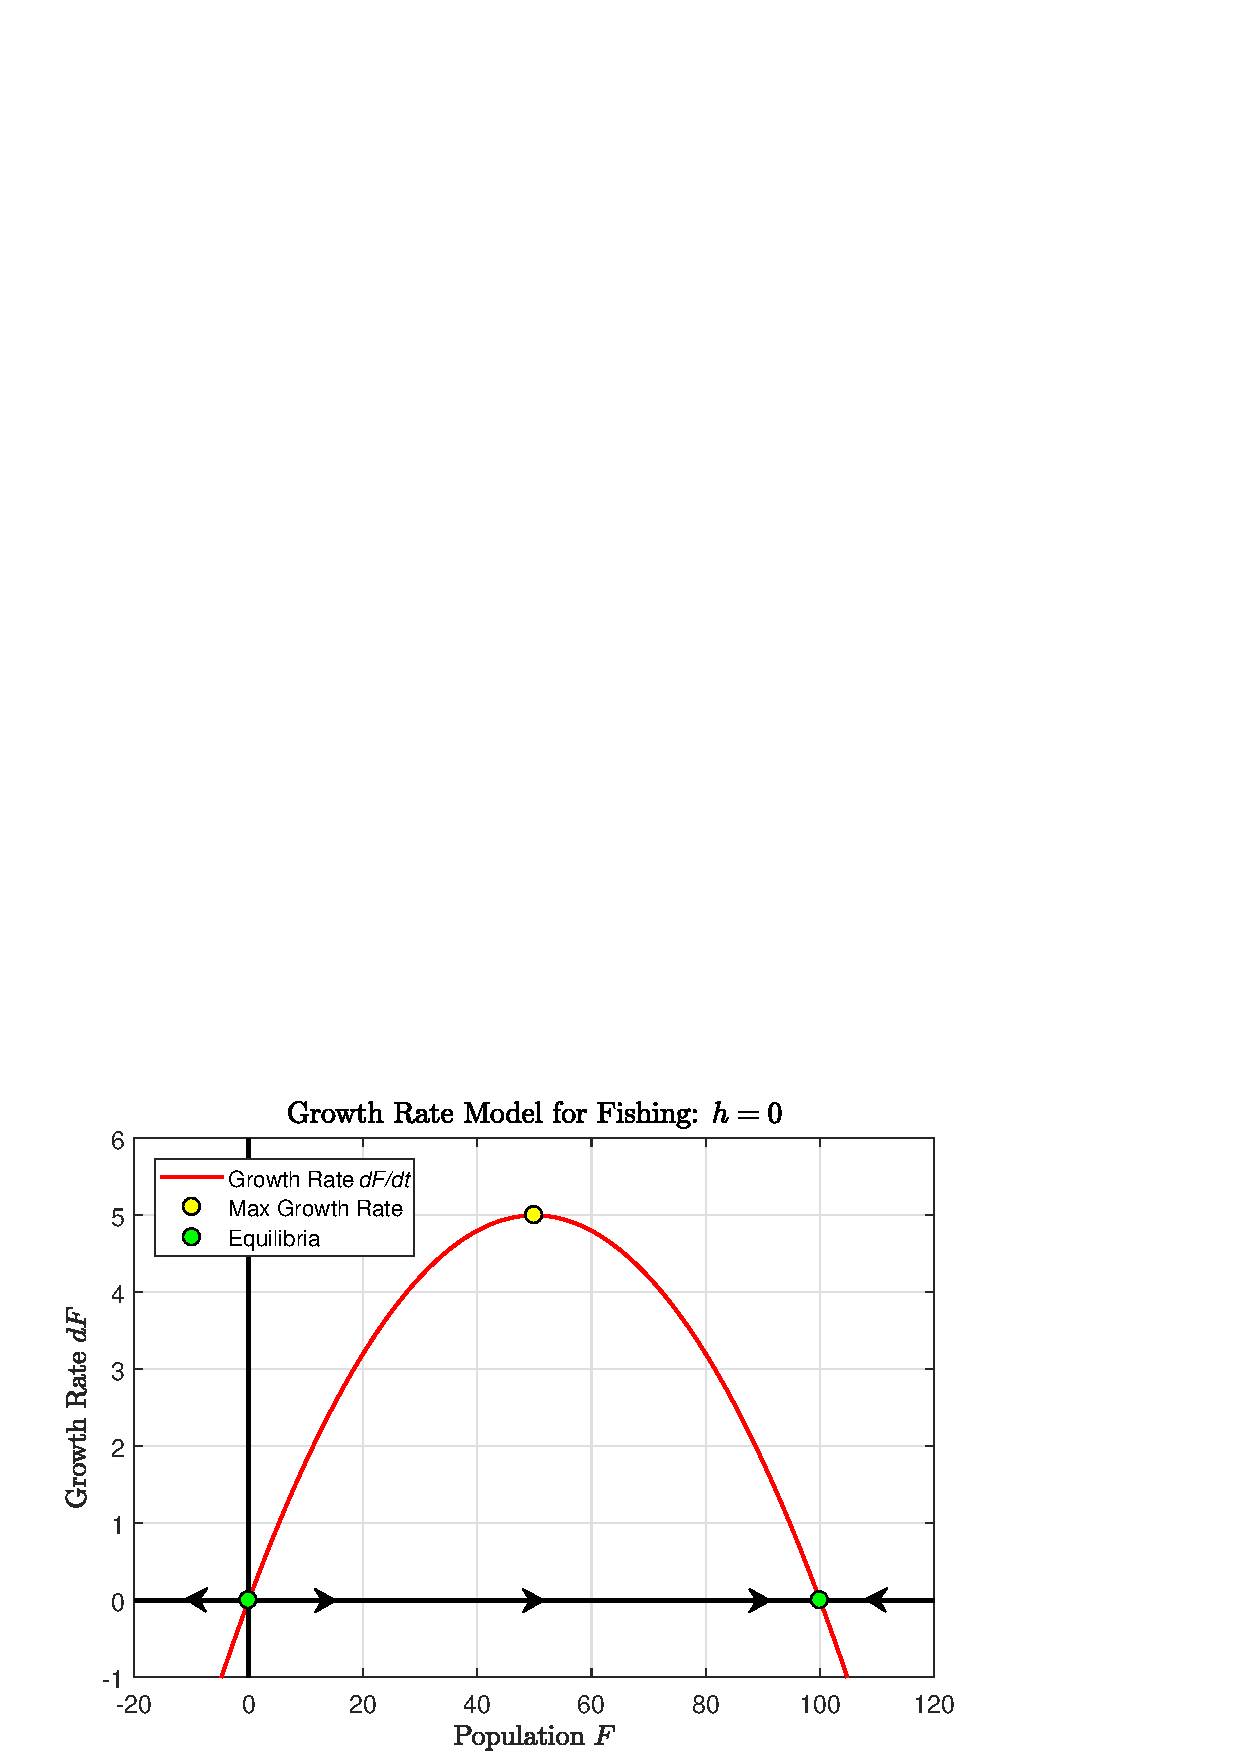
\includegraphics[width=15cm]{f1.png}}
	\caption*{\textbf{Figure i}}
\end{figure}

\subsection*{MATLAB code for enzymatic transformation}

\begin{figure}[H]
	\centering{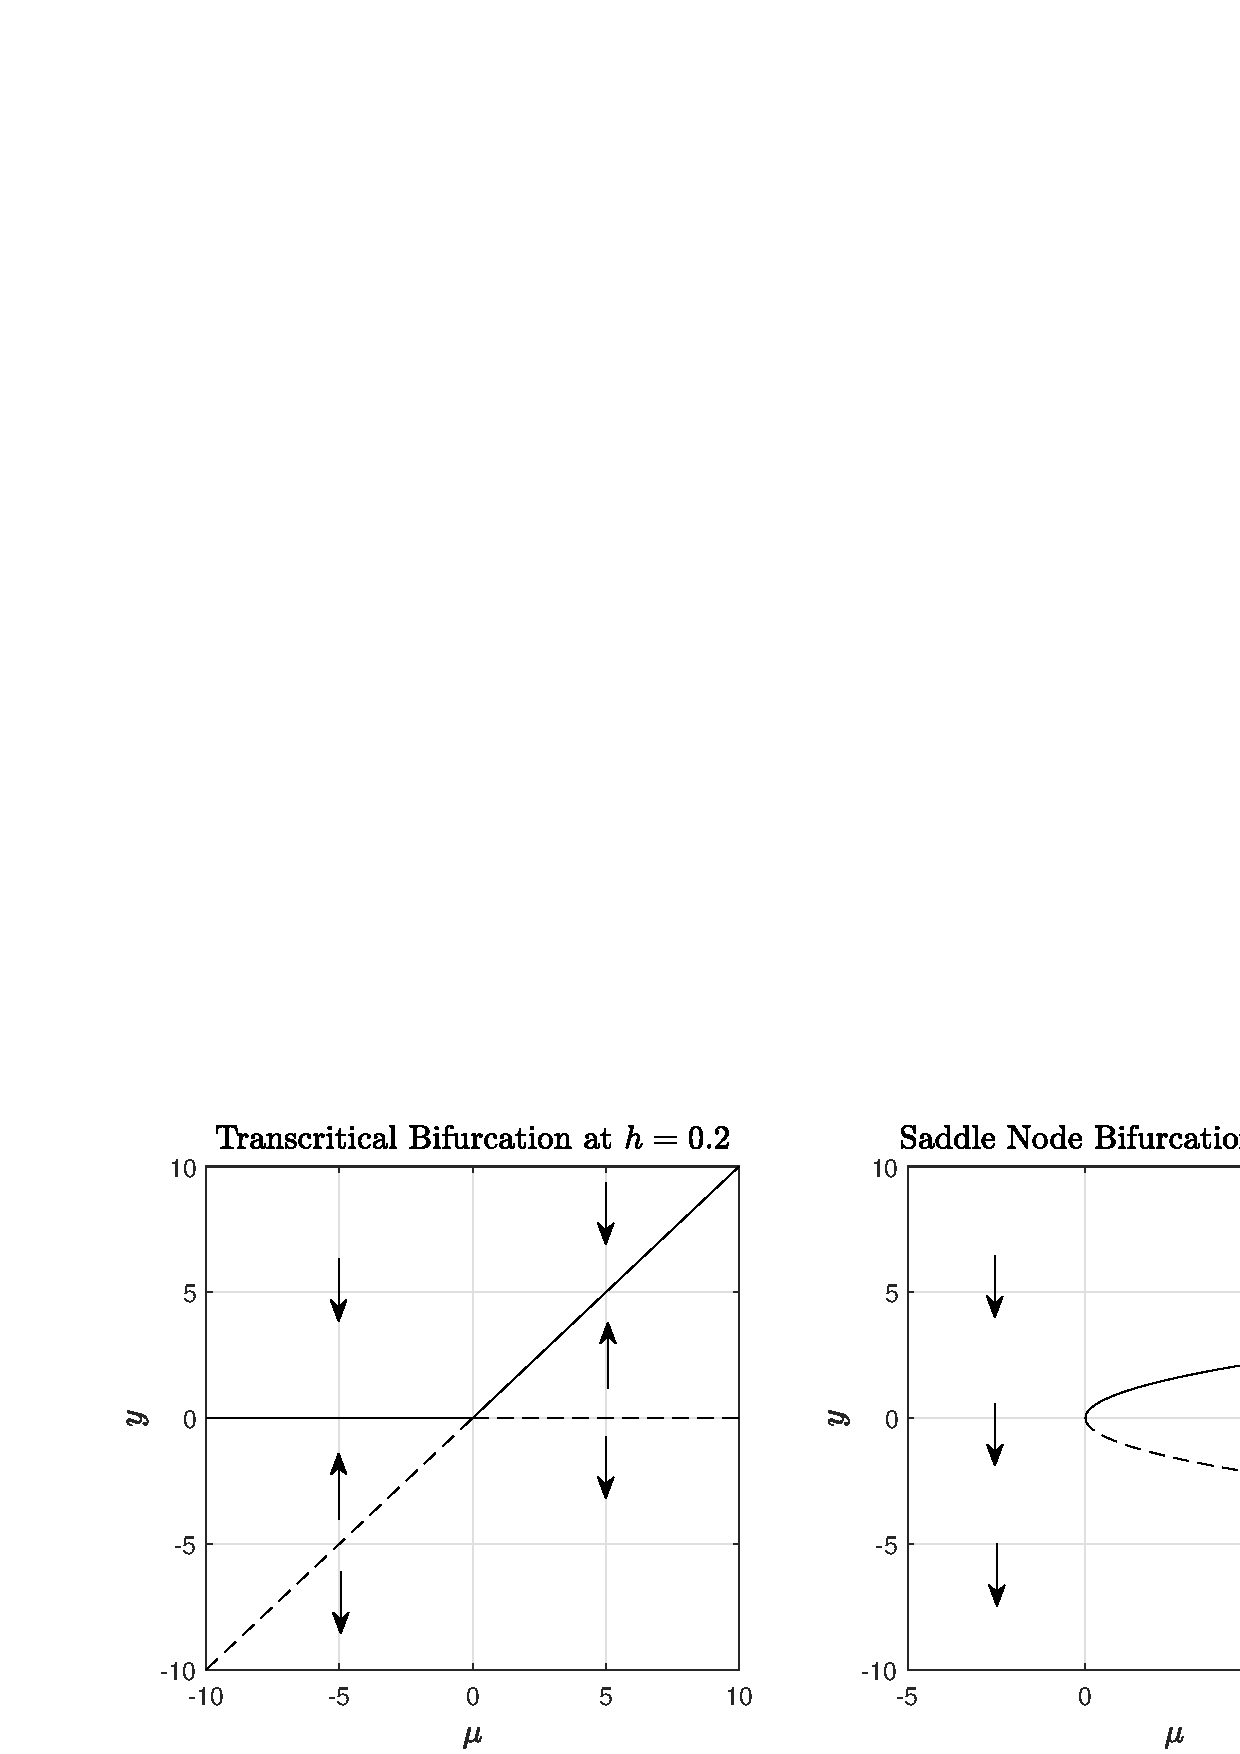
\includegraphics[width=15cm]{f2.png}}
	\caption*{\textbf{Figure ii}}
\end{figure}


\end{document}





































